% Options for packages loaded elsewhere
\PassOptionsToPackage{unicode}{hyperref}
\PassOptionsToPackage{hyphens}{url}
%
\documentclass[
  english,
  man]{apa6}
\usepackage{lmodern}
\usepackage{amssymb,amsmath}
\usepackage{ifxetex,ifluatex}
\ifnum 0\ifxetex 1\fi\ifluatex 1\fi=0 % if pdftex
  \usepackage[T1]{fontenc}
  \usepackage[utf8]{inputenc}
  \usepackage{textcomp} % provide euro and other symbols
\else % if luatex or xetex
  \usepackage{unicode-math}
  \defaultfontfeatures{Scale=MatchLowercase}
  \defaultfontfeatures[\rmfamily]{Ligatures=TeX,Scale=1}
\fi
% Use upquote if available, for straight quotes in verbatim environments
\IfFileExists{upquote.sty}{\usepackage{upquote}}{}
\IfFileExists{microtype.sty}{% use microtype if available
  \usepackage[]{microtype}
  \UseMicrotypeSet[protrusion]{basicmath} % disable protrusion for tt fonts
}{}
\makeatletter
\@ifundefined{KOMAClassName}{% if non-KOMA class
  \IfFileExists{parskip.sty}{%
    \usepackage{parskip}
  }{% else
    \setlength{\parindent}{0pt}
    \setlength{\parskip}{6pt plus 2pt minus 1pt}}
}{% if KOMA class
  \KOMAoptions{parskip=half}}
\makeatother
\usepackage{xcolor}
\IfFileExists{xurl.sty}{\usepackage{xurl}}{} % add URL line breaks if available
\IfFileExists{bookmark.sty}{\usepackage{bookmark}}{\usepackage{hyperref}}
\hypersetup{
  pdftitle={Consistency and variability in the development of children's drawings of object categories},
  pdflang={en-EN},
  pdfkeywords={children's drawings, visual production, tracing, object recognition, visuomotor control},
  hidelinks,
  pdfcreator={LaTeX via pandoc}}
\urlstyle{same} % disable monospaced font for URLs
\usepackage{graphicx,grffile}
\makeatletter
\def\maxwidth{\ifdim\Gin@nat@width>\linewidth\linewidth\else\Gin@nat@width\fi}
\def\maxheight{\ifdim\Gin@nat@height>\textheight\textheight\else\Gin@nat@height\fi}
\makeatother
% Scale images if necessary, so that they will not overflow the page
% margins by default, and it is still possible to overwrite the defaults
% using explicit options in \includegraphics[width, height, ...]{}
\setkeys{Gin}{width=\maxwidth,height=\maxheight,keepaspectratio}
% Set default figure placement to htbp
\makeatletter
\def\fps@figure{htbp}
\makeatother
\setlength{\emergencystretch}{3em} % prevent overfull lines
\providecommand{\tightlist}{%
  \setlength{\itemsep}{0pt}\setlength{\parskip}{0pt}}
\setcounter{secnumdepth}{-\maxdimen} % remove section numbering
% Make \paragraph and \subparagraph free-standing
\ifx\paragraph\undefined\else
  \let\oldparagraph\paragraph
  \renewcommand{\paragraph}[1]{\oldparagraph{#1}\mbox{}}
\fi
\ifx\subparagraph\undefined\else
  \let\oldsubparagraph\subparagraph
  \renewcommand{\subparagraph}[1]{\oldsubparagraph{#1}\mbox{}}
\fi
% Manuscript styling
\usepackage{upgreek}
\captionsetup{font=singlespacing,justification=justified}

% Table formatting
\usepackage{longtable}
\usepackage{lscape}
% \usepackage[counterclockwise]{rotating}   % Landscape page setup for large tables
\usepackage{multirow}		% Table styling
\usepackage{tabularx}		% Control Column width
\usepackage[flushleft]{threeparttable}	% Allows for three part tables with a specified notes section
\usepackage{threeparttablex}            % Lets threeparttable work with longtable

% Create new environments so endfloat can handle them
% \newenvironment{ltable}
%   {\begin{landscape}\begin{center}\begin{threeparttable}}
%   {\end{threeparttable}\end{center}\end{landscape}}
\newenvironment{lltable}{\begin{landscape}\begin{center}\begin{ThreePartTable}}{\end{ThreePartTable}\end{center}\end{landscape}}

% Enables adjusting longtable caption width to table width
% Solution found at http://golatex.de/longtable-mit-caption-so-breit-wie-die-tabelle-t15767.html
\makeatletter
\newcommand\LastLTentrywidth{1em}
\newlength\longtablewidth
\setlength{\longtablewidth}{1in}
\newcommand{\getlongtablewidth}{\begingroup \ifcsname LT@\roman{LT@tables}\endcsname \global\longtablewidth=0pt \renewcommand{\LT@entry}[2]{\global\advance\longtablewidth by ##2\relax\gdef\LastLTentrywidth{##2}}\@nameuse{LT@\roman{LT@tables}} \fi \endgroup}

% \setlength{\parindent}{0.5in}
% \setlength{\parskip}{0pt plus 0pt minus 0pt}

% \usepackage{etoolbox}
\makeatletter
\patchcmd{\HyOrg@maketitle}
  {\section{\normalfont\normalsize\abstractname}}
  {\section*{\normalfont\normalsize\abstractname}}
  {}{\typeout{Failed to patch abstract.}}
\makeatother
\shorttitle{Development of drawing}
\author{Bria Long\textsuperscript{1}, Ying Wang\textsuperscript{2}, Stella Christie\textsuperscript{2}, Michael C. Frank\textsuperscript{1}, \& Judith E. Fan\textsuperscript{3}}
\affiliation{
\vspace{0.5cm}
\textsuperscript{1} Stanford University\\\textsuperscript{2} Tsinghua University\\\textsuperscript{3} University of California, San Diego}
\authornote{

Correspondence concerning this article should be addressed to Bria Long, 450 Jane Stanford Way, Stanford CA 94305. E-mail: bria@stanford.edu}
\keywords{children's drawings, visual production, tracing, object recognition, visuomotor control\newline\indent Word count: X}
\DeclareDelayedFloatFlavor{ThreePartTable}{table}
\DeclareDelayedFloatFlavor{lltable}{table}
\DeclareDelayedFloatFlavor*{longtable}{table}
\makeatletter
\renewcommand{\efloat@iwrite}[1]{\immediate\expandafter\protected@write\csname efloat@post#1\endcsname{}}
\makeatother
\usepackage{csquotes}
\ifxetex
  % Load polyglossia as late as possible: uses bidi with RTL langages (e.g. Hebrew, Arabic)
  \usepackage{polyglossia}
  \setmainlanguage[]{english}
\else
  \usepackage[shorthands=off,main=english]{babel}
\fi

\title{Consistency and variability in the development of children's drawings of object categories}

\date{}

\abstract{
Childen's drawings of common object categories become dramatically more recognziable across development. What are the major factors that explain this developmental change? Here, we examined the degree to which these developmental changes in recognizibility vary across different drawing tasks (i.e.~drawing from observation vs.~from memory), geographical locations (San Jose, US vs.~Beijing, China),and with children's tracing abilities. To do so, we collecting digital drawings of object categories (e.g., cat, airplane) from 4-9 year-olds (N=253). Overall, we show broad consistency in these developmental trajectories acros both drawing tasks and these two geographical locations, and we find that children's tracings abilites are good predictors of the recognizability of the drawings that they produce. In addition, we find that children recruited near Beijing, China producedmore recognizable drawings but showed similar tracing abilities to childen recruited near San Jose, CA. Overall, this work suggests that the developmental trajectory of children's drawings are remarkably consistent and not easily explainable by changes in their visuomotor control.
}

\begin{document}
\maketitle

As humans, we have many powerful tools to externalize what we know, including language and gesture.
One tool that has been transformative for human cognition and culture is graphical representation, which allows people to encode their thoughts in a visible, durable format.
Drawing is an important case study in graphical representation, being a technique that dates back 60,000 years (Hoffmann et al., 2018), well before the emergence of symbolic writing systems, and is practiced in many cultures.

In modern times, drawings are produced prolifically by children from an early age.
Figurative drawings have long provided inspiration for scientists investigating children's emerging cognitive abilities (Minsky \& Papert, 1972), and accordingly a long history of work has examined changes in children's drawings across development (Fury, Carlson, \& Sroufe, 1997; Karmiloff-Smith, 1990; Kellogg, 1969; Piaget, 1929).
Indeed, there appear to be dramatic changes in how children encode diagnostic visual information in their drawings across age; younger children (4-5 years) tend to include fewer cues in their drawings to differentiate between target concepts (e.g., \textit{adult} vs.~\textit{child}) than older children, who enrich their drawings with more diagnostic part (Sitton \& Light, 1992) and relational (Light \& Simmons, 1983) information.
Overall, younger children produce drawings of object categories that are less diagnostic of the categories they are trying to depict (Long, Fan, Chai, \& Frank, 2021; Long, Fan, \& Frank, 2018).

What drives these dramatic changes in children's drawings across development?
A common view is that these changes are driven primarily by children's increasing ability to plan and control their motor movements (Freeman, 1987; Rehrig \& Stromswold, 2018).
While such changes in visuomotor control are clearly important, this view fails to account for other important constraints, such as how well children are able to access previously acquired semantic knowledge about each target concept and maintain this information in working memory during drawing production.
Thus, drawing is a skill that likely also relies on children's evolving perceptual category representations (Dekker, Mareschal, Sereno, \& Johnson, 2011; Long et al., 2018; Natu et al., 2016) as well as their increasing working memory capacity (Pailian, Libertus, Feigenson, \& Halberda, 2016).

One idea is that a principal reason younger children produce less recognizable drawings is because they simply have more difficulty recalling the relevant perceptual features of different categories: that is, when asked to \enquote{draw a {[}rabbit{]}}, they may struggle to conjure up the relevant perceptual details and then hold in mind what rabbits tend to look like.
On this account, providing children with additional perceptual information about different categories -- for example, canonical photographs of typical exemplars -- could help them improve their drawings of these categories, as it does with adults (Fan et al., 2020).
However, prior work also suggests that younger children tend to draw what they know about objects rather than integrate the information in their immediate perceptual experience.\\
For example, when asked to draw from observation, younger children tend to include features that are not visible from their vantage point, yet are diagnostic of category membership (e.g., a handle on a \textit{mug}) (Barrett \& Light, 1976; Bremner \& Moore, 1984), and only omit these features later in development.
Similarly, young children will insist that their nearly identical drawings of different concepts (e.g., balloon and person) unambiguously refer to different things (Bloom \& Markson, 1998).
Thus, an alternative possibility is that only older children may be able to produce more recognizable drawings when provided with canonical exemplars of different categories.
On this account, changes in children's drawings from memory across age may be largely due to other factors beyond changes in memory -- for example, changes in how children represent the diagnostic visual features of each category (Long et al., 2018).

To tease apart these alternatives, we investigated the development of children's ability to produce recognizable drawings of visual concepts when asked to draw from memory (\enquote{Can you draw a {[}rabbit{]}?) and when asked to draw a canonical exemplar from observation (}Can you draw this {[}rabbit{]} as it looks in the picture?") across two different geographical sites (San Jose, USA and Beijing, China).
To do so, we gathered digital drawings from a large sample of children 4-9 years of age in a controlled experimental setting.
While children in different communities may spend more or less time practicing drawing or use different visual conventions to draw (Cohn, 2012; Willats, 2006), most empirical studies on children's drawings have been conducted exclusively on children from the United States -- or focused on differences in educational practices between communities (Huntsinger, Jose, Krieg, \& Luo, 2011; La Voy et al., 2001; Winner, 1989).
In addition, we assessed the degree to which visuomotor development accounts for developmental changes in drawing recognizability by measuring each child's shape tracing abilities.

We had several predictions about the nature of the effects that we would observe. First, we predicted that only older children would be able to use the visual information present in the canonical photographs to improve their drawings, in keeping with accounts of naïve realism and contra a strong account of working memory limitations.
Second, we predicted that we would see convergence in the development of drawing abilities across both geographical sites, with older children becoming progressively better at producing recognizable drawings.
Finally, we predicted that most of the variance across geographical sites in drawing ability would be explainable by differences in visuomotor control, operationalized as performance on a shape tracing task; these primary analyses were pre-registered at \url{https://osf.io/qymjr/}.

\hypertarget{methods}{%
\section{Methods}\label{methods}}

\hypertarget{participants}{%
\subsection{Participants}\label{participants}}

265 participants were recruited from the San Jose Children's Discovery museum, the Palo Alto Junior Museum and Zoo, and preschool and elementary schools outside of Beijing; approximately equal numbers of participants were recruited in Northern California and the Beijing area. Our goal was to recruit 120 children between 4-9 years of age after exclusions (i.e.~20 4-year-olds, 20 5-year-olds, etc.) at each geographical site. In the San Jose based sample, 135 children participated in the experiment; 6 participants were excluded, (3) for skipping more than 6 drawing trials and (3) for scribbling three or more times in a row. Six additional participants were tested but their data was not recorded due to a technical error, and two participants never advanced past the practice trials, leading to a final sample of 121 children. In the Beijing based sample, 132 children participated; an additional 8 participants were tested but their data was not recorded due to a technical error with the remote database. Two 10-year-olds (aged 10 years, 0 months and 10 years, 1 month) were accidentally tested and included in the 9-year-old age group. On average, each child contributed 11.46 to analysis (min 6, max = 12). No additional demographic data was recorded about the participants. This protocol was approved by both the Institutional Review Board at {[}blinded{]} (43992, Development of Children's Drawing Abilities) and the Department of Psychology Ethics Committee at {[}blinded{]} in Beijing, China.

\hypertarget{task-procedure}{%
\subsection{Task Procedure}\label{task-procedure}}

Before beginning, a trained experimenter first told each child \enquote{After this game is over, someone is going to try to recognize what you were trying to draw. So, please draw so that someone else could try what you were trying to draw.} A native English speaker gave these instructions to the San Jose based sample, and a native Mandarin speaker gave a translation of these instructions to the Beijing based sample. The rest of the instructions were given via audio and video cues of native English/Mandarin speakers, respectively; all experimental code, videos, and stimuli are available on the public repository for this project. All children used their fingers to draw on an Ipad Pro (12.9") that was set at a slight angle on a table via a tablet case. All experimental code, videos, and data are available on the public repository for this project.

Children first completed two series of tracing trials to obtain an estimate of their tracing abilities; children were first asked to trace a square and then a complex shape (see Figure \ref{fig:example-tasks}). Children had maximum of 30 seconds to produce their tracings/drawings on all trials, and strokes could not be deleted once drawn; stroke-by-stroke data for each drawing was stored on a remote server.

The primary experimental manipulation was the drawing task that children participated in; each child completed both tasks and the order of tasks was counterbalanced across participants. To elicit drawings from memory, children saw a short video clip where an experimenter said, \enquote{What about a {[}cat{]}? Can you draw a {[}cat{]}?} (exact Mandarin translation has trouble in latex). To elicit drawings from observation, children heard audio of the same experimenter who said, \enquote{What about this {[}cat{]}? Can you draw the {[}cat{]} as it looks in the picture?} (Mandarin translation) while seeing a canonical photograph of each category; this photograph then remained on the screen for the duration of the drawing trial. This photograph was randomly sampled from one of three possible exemplars. Overall, each child completed 2 tracing trials and 12 drawing trials, with six categories randomly assigned to each condition and displayed in a random order. Task examples are shown in Figure \ref{fig:example-tasks}.

\begin{figure}[H]
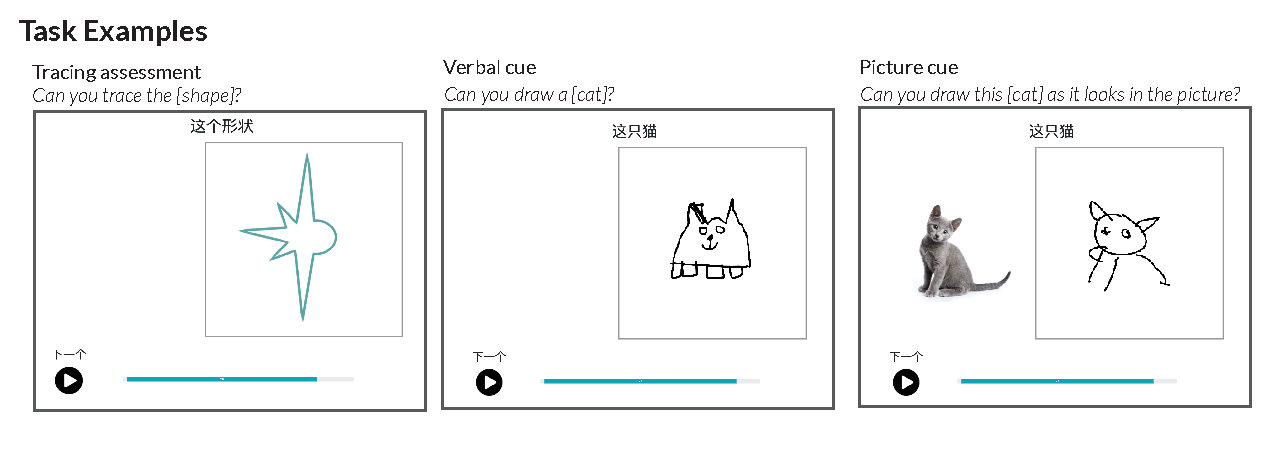
\includegraphics[width=1\linewidth]{figs/task_examples} \caption{Example trials from the tracing assessment and two drawing tasks.}\label{fig:example-tasks}
\end{figure}

\hypertarget{measuring-effort-covariates}{%
\subsection{Measuring effort covariates}\label{measuring-effort-covariates}}

For each drawing trial, children had up to 30 seconds to complete their drawings with their fingers. We recorded both the final drawings and the parameters of each stroke produced by children, allowing us to estimate the amount of time children put into their drawings (e.g., end time of last stroke --- start time of first stroke). As a second measure of effort, we also counted the number of strokes that children put into a given drawing. Finally, we estimated the proportion of the drawing canvas that was filled (e.g., \enquote{ink used}) by computing the proportion of each final drawing that were non-white pixels.

\hypertarget{measuring-tracing-accuracy}{%
\subsection{Measuring Tracing Accuracy}\label{measuring-tracing-accuracy}}

As in (Long et al., 2018), we used an automated procedure for evaluating how accurately participants performed the tracing task, validated against empirical judgments of tracing quality. We decomposed tracing accuracy into two components: a shape error component and a spatial error component. Shape error reflects how closely the participant's tracing matched the contours of the target shape; the spatial error reflects how closely the location, size, and orientation of the participant's tracing matched the target shape.

To compute these error components, we applied an image registration algorithm, AirLab (Sandkühler, Jud, Andermatt, \& Cattin, 2018), to align each tracing to the target shape, yielding an affine transformation matrix that minimized the pixel-wise correlation distance between the aligned tracing, \(T\), and the target shape, \(S\): \(Loss_{NCC} = - \frac{\sum S \cdot T - \sum E(S) E(T)}{N \sum Var(S) Var(T)}\), where \(N\) is the number of pixels in both images. The shape error was defined by the final correlation distance between the aligned tracing and the target shape. The spatial error was defined by the magnitude of three distinct error terms: location, orientation, and size error, derived by decomposing the affine transformation matrix above into translation, rotation, and scaling components, respectively. In sum, this procedure yielded four error values for each tracing: one value representing the shape error (i.e., the pixel-wise correlation distance) and three values representing the spatial error (i.e., magnitude of translation, rotation, scaling components).

We used the same tracing quality ratings to obtained in (Long et al., 2018) to assign weights to each of their error terms; adult observers (\(N\)=70) rated 1325 tracings (i.e., 50-80 tracings per shape per age) and evaluated \enquote{how well the tracing matches the target shape and is aligned to the position of the target shape} on a 5-point scale. An ordinal regression mixed-effects model to predict these 5-point ratings, which contained correlation distance, translation, rotation, scaling, and shape identity (square vs.~star) as predictors, with random intercepts for rater. This model yielded parameter estimates that could then be used to score each tracing in the dataset; we averaged scores for both shapes within session to yield a single tracing score for each participant.

\hypertarget{measuring-drawing-recognizability}{%
\subsection{Measuring drawing recognizability}\label{measuring-drawing-recognizability}}

\hypertarget{human-recognition-scores}{%
\subsubsection{Human recognition scores}\label{human-recognition-scores}}

We assessed the recognizability of each drawing via an online recognition experiment. Adult participants based in the U.S. were recruited via Prolific for a 15 minute experiment,compensated at \$14/hour, and recognized a random subset of around 140 drawings that were balanced with respect to age, category, and site. Each drawing was recognized by 10 participants. Participants were shown a were shown these drawings in a random order and asked \enquote{What does this look like?}. Participants selected an answer from the twelve categories that children were prompted to draw and were were encouraged to guess. No participants were excluded from analysis for missing a catch trial (a free response describing the task that were completing). These binary recognition scores were then averaged across participants to yield a recognition score (e.g., recognized by 80\% of participants) for each drawing.

\hypertarget{automated-recognition-scores}{%
\subsubsection{Automated recognition scores}\label{automated-recognition-scores}}

We used a combination of deep CNN activations and logistic regressions to obtain automated recognition scores, as per our pre-registered protocol. To encode the high-level visual features of each sketch, we used the VGG-19 architecture \cite{simonyan2014very}, a deep convolutional neural network pre-trained on Imagenet classification. We used model activations in the second-to-last layer of this network, which is the first fully connected layer of the network (FC6). Raw feature representations in this layer consist of flat 4096-dimensional vectors, to which we applied channel-wise normalization across all filtered drawings in the dataset. Next, we used these features to train object category decoders. We then trained a 12-way logistic classifier with L2 regularization (tolerance = .1, regularization = .1), and used this classifier to estimate the category label for each drawing in the dataset.To avoid any bias due to imbalance in the distribution of drawings over categories, we randomly under sampled such that there were an equal number of drawings for each combination of geographical site (San Jose, Beijing) and the 12 categories. No additional metadata about the age of the child who produced each sketch was provided to the decoder. This procedure was repeated for each drawing in the dataset, yielding a binary a recognition score for each drawing.

\hypertarget{statistical-models}{%
\subsection{Statistical models}\label{statistical-models}}

To assess our main hypotheses, we fit linear mixed effects models to the human recogniton scores to assess the factors that influenced the recognizability of the drawings that children produced. A first linear mixed effect model was fit to the recognizability scores assigned to each drawing, including fixed effects of children's age (in years), geographical site (San Jose vs.~Beijing), and drawing task (drawing from perception vs.~memory) and the three way interaction between these key variables. We initially planned to include random slopes for the effect of drawing task on each child (as this varied within-subjects), and random slopes for the effect the full three-way interactions between task, age, and site on each category. However, all models with this complicated random effects structure failed to converge, and the reported models the maximal random effects structure that did converge.

In a secondary analysis, we aimed to understand the degree to which any of the above effects were mediated by (1) children's tracing abilities and (2) the amount of effort that children expended while drawings. We thus ran the same main model while also now including fixed effects of children's estimated tracing score (see above), the time children spent drawing (in seconds), the mean intensity of the drawing (i.e.~percentage of non-white pixels), and the number of strokes children used. All predictors were scaled to have a mean of 0 and a standard deviation of 1. Finally, we also assessed the degree to which tracing ability development differed by geographical site, where tracing scores were modeled as a function of age (in years), site, and their interaction, with random intercepts for each participant.

This anlaysis plan was pre-registered at \url{https://osf.io/qymjr/}; however, we had initially planned to use automated recognition scores as our main dependent variable, following prior work (Long et al., 2021); however, we found that these automated recognition scores were only modestly correlated with human recognition scores (\(r\) = 0.40, \(t\) = 0.40, p \textless{} .001); furthermore, descriptive plots of the automated recognition scores revealed a difference between the two drawing tasks that was not evident in the human data. To be conservative, we thus fit all of our models to the human recognition data but have made all model classifications available for future researcs.

\hypertarget{results}{%
\section{Results}\label{results}}

Overall, we found relative consistency in the developmental trajectory of children's drawings. Figure \ref{fig:main-results} shows the recognizability of children's drawings at each age as a function of the drawing task and the geographical site that they were located in; All model coefficients can be found in Table 1. First, we found consistent and steady changes in the recognizability of children's drawings across this age range, replicating prior work with observational datasets collected at a free-standing kiosk (Long et al., 2021). Critically, these changes in recognizability did not depend on the drawing task children completed: children's drawings were equally recognizable when they were asked to \enquote{Draw this rabbit as it looks in the picture} and they were simply asked \enquote{What about a rabbit? Can you draw a rabbit.} While we anticipated that older children might produce more recognizable drawings when drawing from observation -- as do adults when presented with canonical photographs of object categories (Yang \& Fan, 2021) -- this was not the case.

However, we did observe a main effect of geographical site: Children who were recruited near Beijing, China tended to produce more recognizable drawings than children who were recruited near San Jose, USA. In a second set of analyses, we aimed to understand the nature of this difference in recognizability. We hypothesized that any differences in the recognizability of children's drawings across sites would be mediated by the amount of effort children expended while drawing or their tracing abilities. We thus first examined how effort and tracing abilities varied across task, age, and geographical location. Figure \ref{fig:effort-covariates} shows three effort covariates - average intensity, number of strokes used, and time spent drawing -- measured for each drawing as a function of children's age, drawing task, and geographical site: effort covariates measured for each drawing; children tended to spend more time drawing when asked to draw \enquote{the {[}rabbit{]} as it looks in the picture}, and children recruited outside Beijing tended to spend more time drawing overall. In contrast, children's tracing abilities did not vary across geographical site: Figure \ref{fig:tracing} shows the average tracing score at each age at each site. While children's tracing abilities increased steadily with age, as in prior work (Long et al., 2021), children recruited at both sites produced equally good shape tracings.

Next, we included children's average tracing scores and effort covariates measured for each drawing (average intensity, number of strokes used, and time spent drawing) as fixed effects into a second linear mixed-effects model with the same fixed and random effects structure as used above. If these effort covariates accounted the differences between sites that we observed, we reasoned that we should no longer observe a main effect of geographical location on drawing recognizability. Contra this hypothesis, however, we still observed a significant effect of geographical site (see Table 2), despite the fact that individual children's tracing abilities were strong predictors of how recognizable their drawings were. In addition, the amount of time a child spent drawing was a significant negative predictor of recognizability -- indicating that the amount of effort that children expended did not necessarily result in a drawing that was more recognizable to others.

Thus, these results suggest that these two groups of children differ in their ability to produce recognizable drawings of object categories in a way that is not esaily explainable by effort covariates or tracing abilities, contra previous accounts. In a third set of analyses, we examined how the developmental trajectory of the recognizability of children's drawings may differ for different object categories. Intuitively, some object categories (e.g., cat) may be easier to draw than others (e.g., watch), resulting in shallower or steeper changes in recognizability over age. However, we had no strong hypotheses about how these trajectories might additionally vary with geographical locations.

Figure \ref{fig:item-effects} shows the recognizability of children's drawings for each of the 12 categories a function of geographical location and children's age and reveal considerable variability. For example, certain categories (e.g., cats and rabbits) were overall more difficult for children to depict such that they were distinct from one another, particularly for younger children. In addition, children recruited near Beijing produced more recognizable drawings of certain categories at all ages -- including airplanes, birds, and rabbits -- while older children recruited near San Jose produced more recognizable drawings of bikes. Figure \ref{fig:example-drawings} shows recognizable, randomly sampled example drawings from 6-year-olds at each category, site, and condition.

\begin{verbatim}
## Warning: Removed 690 rows containing missing values (geom_point).
\end{verbatim}

\begin{figure}[H]

{\centering \includegraphics[width=\textwidth]{Manuscript_June2021_files/figure-latex/main-results-1} 

}

\caption{Proportion of drawings recognized as a function of the age of the child who completed each drawing, the geographical site they were tested at (San Jose vs. Beijing), and the type of drawing task they completed. Individual data points represent drawings within each condition by an individual participant and are slightly jittered. Error bars show bootstrapped 95 percent cofnidence intervals.}\label{fig:main-results}
\end{figure}

\begin{table}[ht]
\centering
\begin{tabular}{rrrrrr}
  \hline
 & Estimate & Std. Error & df & t value & Pr($>$$|$t$|$) \\
  \hline
Intercept & 0.73 & 0.02 & 31.62 & 34.74 & 0.000 \\
  Task & -0.02 & 0.02 & 17.29 & -0.87 & 0.397 \\
  Age & 0.17 & 0.02 & 373.04 & 11.21 & 0.000 \\
  Site & 0.05 & 0.02 & 385.12 & 2.39 & 0.017 \\
  Task*Age & -0.02 & 0.01 & 2622.52 & -1.47 & 0.141 \\
  Task*Site & -0.00 & 0.02 & 2631.48 & -0.20 & 0.842 \\
  Age*Site & -0.00 & 0.02 & 388.66 & -0.06 & 0.951 \\
  Task*Age*Site & 0.00 & 0.02 & 2639.46 & 0.21 & 0.834 \\
   \hline
\end{tabular}
\caption{Table 1. Model coefficients from a linear mixed mode predicting the recognizability of each drawing for the main experimental contrasts.}
\end{table}

\begin{table}[ht]
\centering
\begin{tabular}{rrrrrr}
  \hline
 & Estimate & Std. Error & df & t value & Pr($>$$|$t$|$) \\
  \hline
Intercept & 0.72 & 0.02 & 34.02 & 37.49 & 0.000 \\
  Task & -0.02 & 0.02 & 17.55 & -1.19 & 0.249 \\
  Age & 0.14 & 0.02 & 376.68 & 9.30 & 0.000 \\
  Site & 0.07 & 0.02 & 459.46 & 3.58 & 0.000 \\
  Est. tracing score & 0.06 & 0.01 & 249.21 & 5.71 & 0.000 \\
  Avg. intensity & 0.01 & 0.01 & 2839.40 & 1.90 & 0.058 \\
  Draw duration & -0.03 & 0.01 & 1692.69 & -3.42 & 0.001 \\
  Number of strokes & 0.03 & 0.01 & 2655.21 & 4.67 & 0.000 \\
  Task*Age & -0.02 & 0.01 & 2623.63 & -1.72 & 0.086 \\
  Task\&Site & -0.01 & 0.02 & 2630.59 & -0.45 & 0.655 \\
  Age*Site & -0.01 & 0.02 & 415.59 & -0.74 & 0.462 \\
  Task*Age*Site & 0.00 & 0.02 & 2638.72 & 0.18 & 0.858 \\
   \hline
\end{tabular}
\caption{Table 2. Model coefficients from a linear mixed mode predicting the recognizability of each drawing as a function the both the main experimental contrasts (task, site, and age) as well as several effort covariates and individual's estimates tracing abilities.}
\end{table}

\begin{figure}[H]

{\centering \includegraphics[width=\textwidth]{Manuscript_June2021_files/figure-latex/effort-covariates-1} 

}

\caption{Effort covariates measured during the drawing task -- amount of time spent drawing, amount of 'ink' used, and number of strokes used -- as function of the age of the child who completed each drawing, the geographical site they were tested at (San Jose vs. Beijing), and the type of drawing task they completed. Error bars show bootstrapped 95 percent cofnidence intervals.}\label{fig:effort-covariates}
\end{figure}

\begin{verbatim}
## Warning: Removed 12 rows containing missing values (geom_point).
\end{verbatim}

\begin{figure}[H]

{\centering \includegraphics[width=\textwidth]{Manuscript_June2021_files/figure-latex/tracing-1} 

}

\caption{Average tracing scores across age and site; each dot represents an average tracing score obtained for each participant and are slightly jittered. Error bars represent bootstrapped 95 percent confidence intervals.}\label{fig:tracing}
\end{figure}
\begin{figure}[H]
\includegraphics[width=1\linewidth]{figs/example_drawings} \caption{Randomly sampled, highly recognized drawings for each task, category, and geographical site made by 6-year-old children.}\label{fig:example-drawings}
\end{figure}

\begin{verbatim}
## Warning: Removed 16 rows containing missing values (geom_smooth).
\end{verbatim}

\begin{figure}[H]

{\centering \includegraphics[width=\textwidth]{Manuscript_June2021_files/figure-latex/item-effects-1} 

}

\caption{Developmental trajectory of drawing recognizability for each category and for each geographical site. Error bars represent 95 percent bootstrapped confidence intervals.}\label{fig:item-effects}
\end{figure}

\hypertarget{discussion}{%
\section{Discussion}\label{discussion}}

Here, we examined the consistency and variability in the devleopmental trajectory of children's drawings across two different drawing tasks and geographical locations. We

\hypertarget{acknowledgements}{%
\section{Acknowledgements}\label{acknowledgements}}

We thank Yi Feng and Megan Merrick for assistance with data collection, with whom this project would have not been possible. We also gratefully acknowledge the San Jose Children's Discovery Museum for their collaboration. We are also thankful to all of the parents at XX and XX preschool whose children participated. We also thank the members of the Stanford Language and Cognition lab for their feedback. This work was funded by an NSF SPRF-FR Grant \#1714726 to BLL and a Jacobs Foundation Fellowship to MCF.

\newpage

\hypertarget{references}{%
\section{References}\label{references}}

\begingroup
\setlength{\parindent}{-0.5in}
\setlength{\leftskip}{0.5in}

\hypertarget{refs}{}
\leavevmode\hypertarget{ref-barrett1976symbolism}{}%
Barrett, M., \& Light, P. (1976). Symbolism and intellectual realism in children's drawings. \emph{British Journal of Educational Psychology}, \emph{46}(2), 198--202.

\leavevmode\hypertarget{ref-bloom1998intention}{}%
Bloom, P., \& Markson, L. (1998). Intention and analogy in children's naming of pictorial representations. \emph{Psychological Science}, \emph{9}(3), 200--204.

\leavevmode\hypertarget{ref-bremmer1984prior}{}%
Bremner, J. G., \& Moore, S. (1984). Prior visual inspection and object naming: Two factors that enhance hidden feature inclusion in young children's drawings. \emph{British Journal of Developmental Psychology}, \emph{2}(4), 371--376.

\leavevmode\hypertarget{ref-cohn2012explaining}{}%
Cohn, N. (2012). Explaining ``i can't draw'': Parallels between the structure and development of language and drawing. \emph{Human Development}, \emph{55}(4), 167--192.

\leavevmode\hypertarget{ref-dekker2011dorsal}{}%
Dekker, T., Mareschal, D., Sereno, M. I., \& Johnson, M. H. (2011). Dorsal and ventral stream activation and object recognition performance in school-age children. \emph{NeuroImage}, \emph{57}(3), 659--670.

\leavevmode\hypertarget{ref-fan2020relating}{}%
Fan, J. E., Wammes, J. D., Gunn, J. B., Yamins, D. L., Norman, K. A., \& Turk-Browne, N. B. (2020). Relating visual production and recognition of objects in human visual cortex. \emph{Journal of Neuroscience}, \emph{40}(8), 1710--1721.

\leavevmode\hypertarget{ref-freeman1987current}{}%
Freeman, N. H. (1987). Current problems in the development of representational picture-production. \emph{Archives de Psychologie}.

\leavevmode\hypertarget{ref-fury1997children}{}%
Fury, G., Carlson, E. A., \& Sroufe, A. (1997). Children's representations of attachment relationships in family drawings. \emph{Child Development}, \emph{68}(6), 1154--1164.

\leavevmode\hypertarget{ref-hoffmann2018u}{}%
Hoffmann, D. L., Standish, C. D., Garcia-Diez, M., Pettitt, P. B., Milton, J., Zilhão, J., \ldots{} others. (2018). U-th dating of carbonate crusts reveals neandertal origin of iberian cave art. \emph{Science}, \emph{359}(6378), 912--915.

\leavevmode\hypertarget{ref-huntsinger2011cultural}{}%
Huntsinger, C. S., Jose, P. E., Krieg, D. B., \& Luo, Z. (2011). Cultural differences in chinese american and european american children's drawing skills over time. \emph{Early Childhood Research Quarterly}, \emph{26}(1), 134--145.

\leavevmode\hypertarget{ref-karmiloff1990constraints}{}%
Karmiloff-Smith, A. (1990). Constraints on representational change: Evidence from children's drawing. \emph{Cognition}, \emph{34}(1), 57--83.

\leavevmode\hypertarget{ref-kellogg1969analyzing}{}%
Kellogg, R. (1969). \emph{Analyzing children's art}. National Press Books Palo Alto, CA.

\leavevmode\hypertarget{ref-la2001children}{}%
La Voy, S. K., Pedersen, W. C., Reitz, J. M., Brauch, A. A., Luxenberg, T. M., \& Nofsinger, C. C. (2001). Children's drawings: A cross-cultural analysis from japan and the united states. \emph{School Psychology International}, \emph{22}(1), 53--63.

\leavevmode\hypertarget{ref-light1983effects}{}%
Light, P., \& Simmons, B. (1983). The effects of a communication task upon the representation of depth relationships in young children's drawings. \emph{Journal of Experimental Child Psychology}, \emph{35}(1), 81--92.

\leavevmode\hypertarget{ref-long2021parallel}{}%
Long, B., Fan, J., Chai, Z., \& Frank, M. C. (2021). Parallel developmental changes in children's drawing and recognition of visual concepts.

\leavevmode\hypertarget{ref-long2018drawings}{}%
Long, B., Fan, J., \& Frank, M. C. (2018). Drawings as a window into developmental changes in object representations. In \emph{Proceedings of the 40th annual meeting of the cognitive science society}.

\leavevmode\hypertarget{ref-minsky1972artificial}{}%
Minsky, M., \& Papert, S. (1972). \emph{Artificial intelligence progress report}. Cambridge, MA, USA: Massachusetts Institute of Technology.

\leavevmode\hypertarget{ref-natu2016development}{}%
Natu, V. S., Barnett, M. A., Hartley, J., Gomez, J., Stigliani, A., \& Grill-Spector, K. (2016). Development of neural sensitivity to face identity correlates with perceptual discriminability. \emph{Journal of Neuroscience}, \emph{36}(42), 10893--10907.

\leavevmode\hypertarget{ref-pailian2016visual}{}%
Pailian, H., Libertus, M. E., Feigenson, L., \& Halberda, J. (2016). Visual working memory capacity increases between ages 3 and 8 years, controlling for gains in attention, perception, and executive control. \emph{Attention, Perception, \& Psychophysics}, \emph{78}(6), 1556--1573.

\leavevmode\hypertarget{ref-piaget1929child}{}%
Piaget, J. (1929). The child's concept of the world. \emph{Londres, Routldge \& Kegan Paul}.

\leavevmode\hypertarget{ref-rehrig2018does}{}%
Rehrig, G., \& Stromswold, K. (2018). What does the dap: IQ measure?: Drawing comparisons between drawing performance and developmental assessments. \emph{The Journal of Genetic Psychology}, \emph{179}(1), 9--18.

\leavevmode\hypertarget{ref-sandkuhler2018}{}%
Sandkühler, R., Jud, C., Andermatt, S., \& Cattin, P. C. (2018). AirLab: Autograd image registration laboratory. \emph{arXiv Preprint arXiv:1806.09907}.

\leavevmode\hypertarget{ref-sitton1992drawing}{}%
Sitton, R., \& Light, P. (1992). Drawing to differentiate: Flexibility in young children's human figure drawings. \emph{British Journal of Developmental Psychology}, \emph{10}(1), 25--33.

\leavevmode\hypertarget{ref-willats2006making}{}%
Willats, J. (2006). \emph{Making sense of children's drawings}. Psychology Press.

\leavevmode\hypertarget{ref-winner1989can}{}%
Winner, E. (1989). How can chinese children draw so well? \emph{Journal of Aesthetic Education}, \emph{23}(1), 41--63.

\leavevmode\hypertarget{ref-yang2021visual}{}%
Yang, J., \& Fan, J. E. (2021). Visual communication of object concepts at different levels of abstraction. \emph{arXiv Preprint arXiv:2106.02775}.

\endgroup

\end{document}
